% Gemini theme
% https://github.com/anishathalye/gemini

\documentclass[final, 16pt]{beamer}

% ====================
% Packages
% ====================
%\usepackage[x11names]{xcolor} % use color for the horizontal line
\usepackage[T1]{fontenc}
\usepackage{lmodern}
\usepackage[size=custom,width=38.1,height=54.2,scale=0.42]{beamerposter}
\usetheme{gemini}
\usecolortheme{gemini}
\usepackage{graphicx}
\usepackage{booktabs}
\usepackage{tikz}
\usepackage{pgfplots}
\usepackage[square,sort,comma,numbers]{natbib} % for simplify the format of the references
\usepackage{tikz} % for adding the logo
% \usepackage{caption} % for caption font of the table
\setbeamertemplate{caption}[numbered]
\setbeamerfont{caption}{size=\large}

% ====================
% Lengths
% ====================

% If you have N columns, choose \sepwidth and \colwidth such that
% (N+1)*\sepwidth + N*\colwidth = \paperwidth
\newlength{\sepwidth}
\newlength{\colwidth}
\setlength{\sepwidth}{0.025\paperwidth}
\setlength{\colwidth}{0.45\paperwidth}

\newcommand{\separatorcolumn}{\begin{column}{\sepwidth}\end{column}}

% ====================
% Title
% ====================

\title{Mining relationships between food groups, eating time slots\\ and diabetes status in adults from UK NDNS RP}

\author{Luigi Palla \inst{1} \and Chaochen Wang \inst{2} \and Marta Gruszka-Goh \inst{1} \and Suzana Almoosawi \inst{3}}

\institute[shortinst]{\inst{1} Dept Medical Statistics, LSHTM, London, UK; \samelineand \inst{2} Dept Public Health, Aichi Medical University, Aichi, Japan \samelineand \\ \inst{3} Brain, Performance and Nutrition Research Centre, Northumbria University, Newcastle, UK}

% ====================
% Body
% ====================
\pgfplotsset{compat=1.16}
\begin{document}

% logos are added as follows:

\addtobeamertemplate{headline}{} 
{
	\begin{tikzpicture}[remember picture,overlay] 
%	\node [anchor=north east, inner sep=3cm] at (current page.north east) {\includegraphics[height=5cm]{Fig/LSHTM-logo-trans-white.eps}}; 
    \node [anchor=north east, inner sep=3.3cm] at ([xshift=2.5cm,yshift=1.3cm]current page.north east)     {\includegraphics[height=2.5cm]{Fig/LSHTM-logo-trans-white.eps}}; 
	\end{tikzpicture} 
}

\addtobeamertemplate{headline}{} 
{
	\begin{tikzpicture}[remember picture,overlay] 
	%	\node [anchor=north east, inner sep=3cm] at (current page.north east) {\includegraphics[height=5cm]{Fig/LSHTM-logo-trans-white.eps}}; 
	\node [anchor=north west, inner sep=3.6cm] at ([xshift=-2.7cm,yshift=1.5cm]current page.north west) {\includegraphics[height=2.5cm]{Fig/amu-logo-trans-white.eps}}; %{\includegraphics[height=6.6cm]{Fig/amu-logo-trans-green.eps}};  
	\end{tikzpicture} 
}

\addtobeamertemplate{headline}{} 
{
	\begin{tikzpicture}[remember picture,overlay] 
	%	\node [anchor=north east, inner sep=3cm] at (current page.north east) {\includegraphics[height=5cm]{Fig/LSHTM-logo-trans-white.eps}}; 
	\node [anchor=north west, inner sep=3.6cm] at ([xshift=0.5cm,yshift=1.5cm]current page.north west) {
\includegraphics[height=2.5cm]{Fig/suzana-logo-trans-white.eps}}; \end{tikzpicture} 
}



\begin{frame}[t]
\begin{columns}[t]
\separatorcolumn

\begin{column}{\colwidth}
    \vskip-2.45ex
  \begin{block}{Introduction}

    \vskip-1.45ex
    \begin{itemize}
	\item The timing of energy/nutrient intake has been previously shown to be associated with obesity and diabetes \cite{Almoosawi2019Chrono};
	\item Recently derived diurnal patterns of energy/carbohydrate intake suggested the potential interplay of circadian biology and social behaviour contributing to obesity \cite{Palla2019};
	% \item Evening intake of energy is positively associated with incidence of hypertension, and overweight/obesity \cite{Almoosawi2013,almoosawi2016chrono}.
  \item AIM:Characterise the relationship between food groups and the time of day when they are eaten, how such relationships vary by type 2 diabetes status are still left unknown.
\end{itemize}
    % \vskip-1.45ex



% Recent evidence suggested that there are three types of eaters \textbf{(grazers, early eaters, and late eaters)} according to the timing of energy consumption \cite{leech2017temporal,mansukhani2018investigating}. However, the temporal eating patterns were based on averaging the total energy intake  measured in the questionnaires and therefore \textbf{could not capture the day-to-day variation in eating patterns}. Furthermore, most previous studies have focused on describing temporal patterns of energy intake, \textbf{without considering the timing of macro-nutrient intake}.

%    \vskip-1.45ex
%%\begin{itemize}
%	\item 
%	\item 
%	
%%	Besides they were focussed on total energy \textbf{so would not provide any clue of the temporal eating patterns specifically for nutrient intake}.
%	%	\item Shift workers have a higher risk of developing T2D \cite{pan2011rotating}. 
%%\end{itemize}
%\vskip-1.45ex

%%
%However, the temporal eating patterns were based only on averaging the total energy intake measured by 1 or 2 24-hour dietary recalls \cite{leech2017temporal} or 3 to 4 days' diet diary \cite{mansukhani2018investigating} and therefore \textbf{could not capture the day-to-day variation in eating patterns}, and \textbf{neither could it provide any clue of the temporal patterns specifically for nutrient intake}. 

%This is mainly due to limitations in the FFQ often used in observational studies and the lack of understanding of statistical techniques that can capture the complexity of eating patterns across the day. 

% This study aims at finding both time and quantity eating patterns specifically for carbohydrate (CH) intake in UK adults.


  \end{block}


   \vskip-4.25ex
  \begin{block}{Data and Methodology}
    \vskip-2.15ex

\begin{itemize}
	\item National Diet and Nutrition Survey Rolling Programme (NDNS RP, 2008-2017) included 6802 adults (2810 men and 3992 women) aged 19 or older in the UK, and their 749,026 food recordings collected by a 4-day-diary.
	\item Time of the day was categorized into 7 slots: 6-9 am, 9-12 noon, 12-2 pm, 2-5 pm, 5-8 pm, 8-10 pm and 10 pm-6 am; foods recorded were categorised in one of 60 standard food groups.
	\item The derived contingency table cross-classifying 60 food groups with the 7 time slots were analyzed by Correspondence Analysis (CA). Biplots graphically displaying the association were derived for all adults combined and separately by diabetes status.
\end{itemize}
\vskip-2.85ex

\begin{table}
% \captionsetup{font=large}
\centering
% \captionof{table}{Definition of Type 2 Diabetes.} \label{tab:title2} 
\caption{\label{tab:tab1}Definition of Type 2 Diabetes (T2D).}
\vskip-0.85ex
\small
\begin{tabular}{lcccc}
\toprule
\textbf{Diabetes status} & \textbf{Self-reported} & \textbf{Glucose (mmol/L)} & \textbf{HbA1c (\%)} & \textbf{n} \\ \midrule
No diabetes              & No                     & $<$ 6.10                   & $<$ 6.5          & 2626          \\
Pre-diabetes             & No                     & 6.10 $\sim$ 6.99            & --              &   133        \\
Undiagnosed              & No                     & $\geqslant$ 7.00           & $\geqslant$ 6.5  &   99        \\
Diagnosed                & Yes                    & --                        & --                &   227       \\ 
Missing                 & NA                      & NA                        & NA                &  3717 \\ \bottomrule
\end{tabular}
\end{table}
\vskip-2.45ex


\begin{itemize}
	
	\item The odds ratio estimate was derived of consuming the unhealthy food groups (the ones flagged by CA) later in the day compared to earlier in the day, by logistic regression models accounting for repeated measures (food entries) from the same individual.

\end{itemize}
 \vskip-1.45ex
 
% Please add the following required packages to your document preamble:
% \usepackage{booktabs}
  \end{block}

\vskip-2.65ex
  \begin{block}{Results}
\vskip-2.45ex
    \begin{figure}
      \centering
      \caption{Biplot for CA of food groups and time slots among non-diabetics.}
      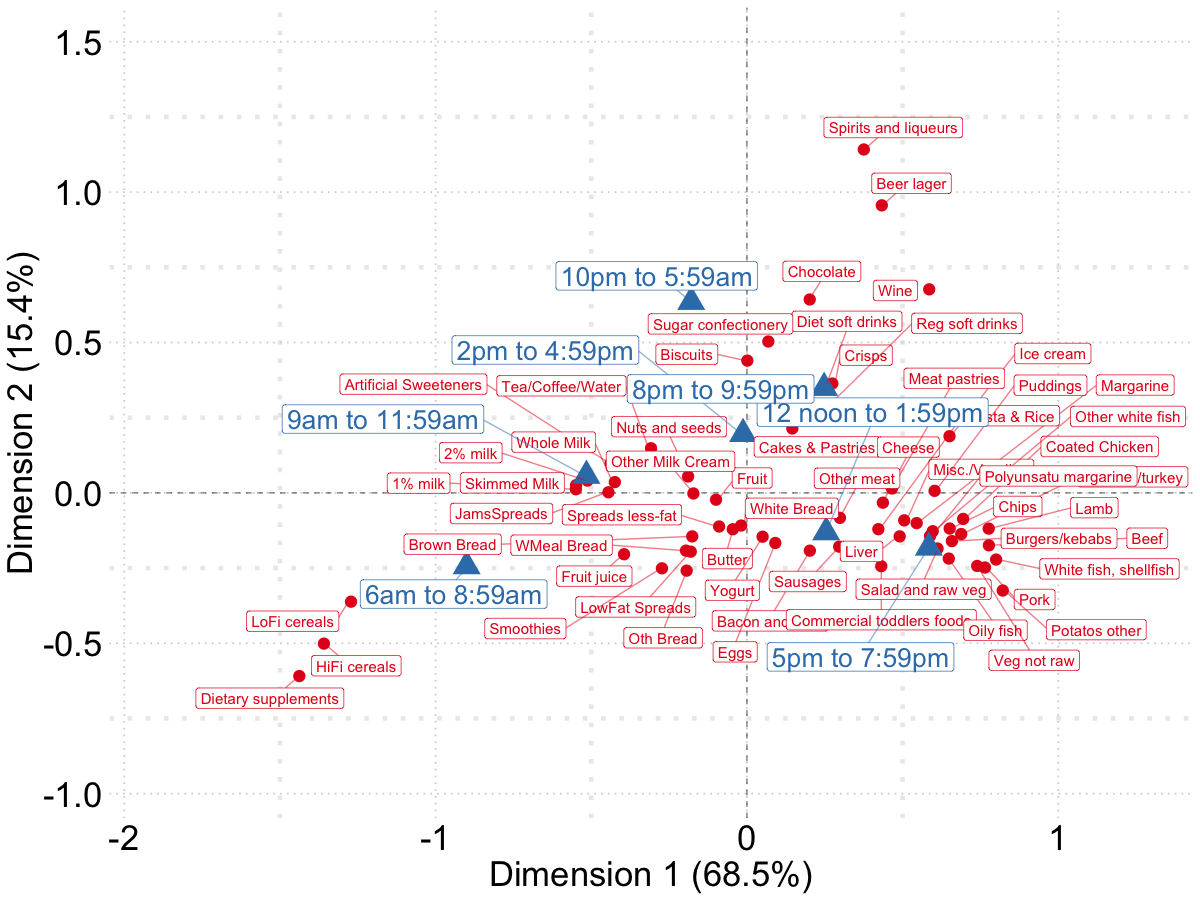
\includegraphics[width=0.88\textwidth]{Fig/F60T7_nonDM.png}	\vskip-2.45ex
      \label{fig:NonDM}
    \end{figure}
\vskip-1ex

\begin{figure}
      \centering
      \caption{Biplot for CA of food groups and time slots among diabetics.}
      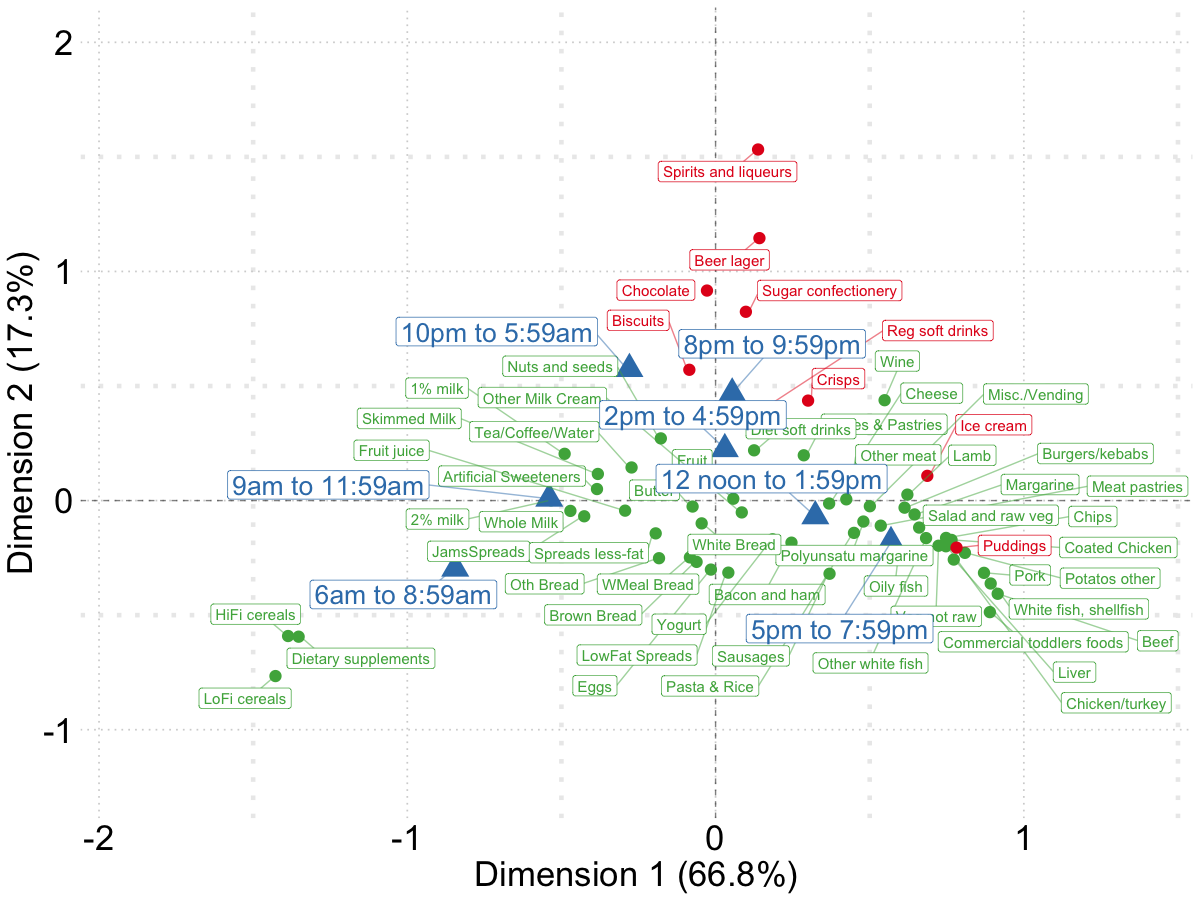
\includegraphics[width=0.88\textwidth]{Fig/F60T7_DM.png}	\vskip-2.45ex
      \label{fig:DM}
    \end{figure}
    
  \end{block}

\end{column}

\separatorcolumn

\begin{column}{\colwidth}
  \begin{block}{}

    \begin{figure}
      \centering
      \caption{Biplot for CA of food groups and time slots among undiagnosed diabetics.}
      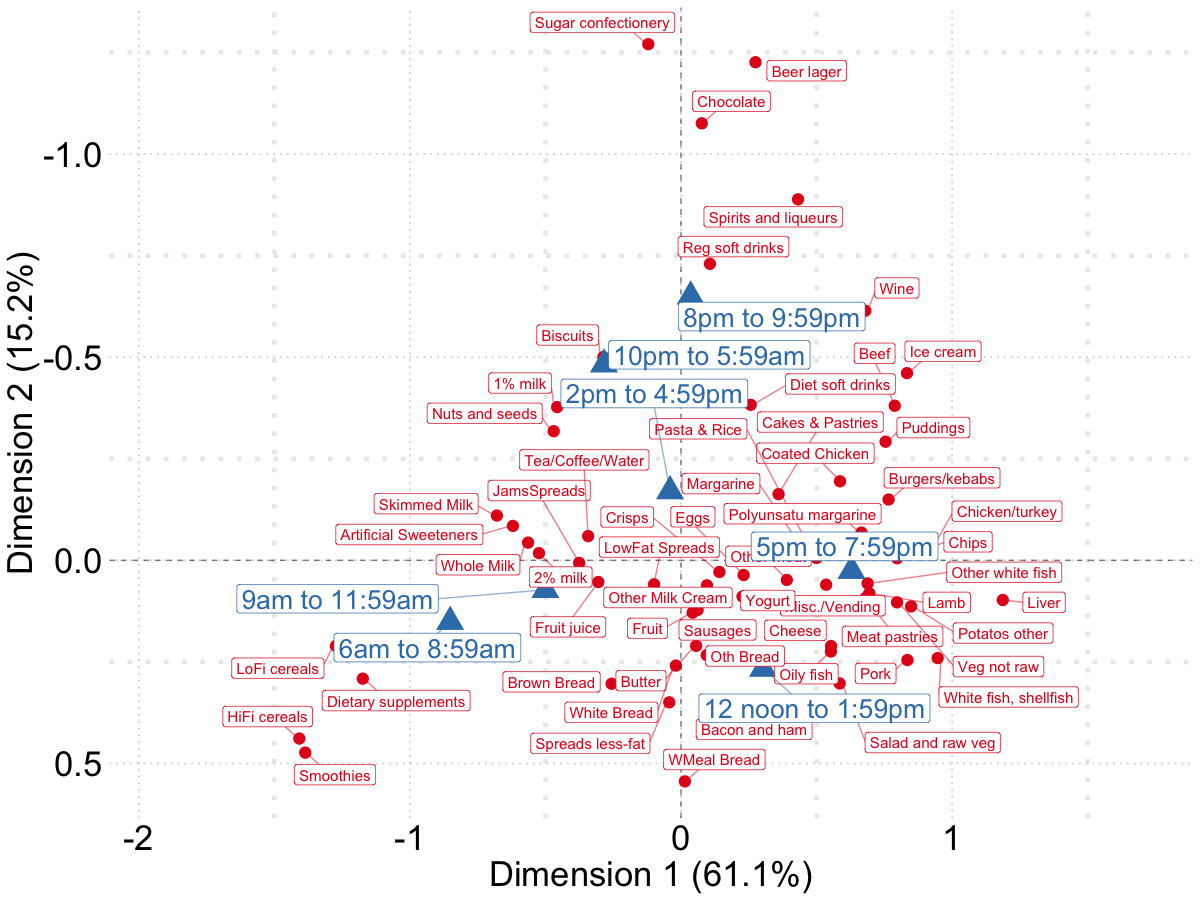
\includegraphics[width=0.88\textwidth]{Fig/F60T7_UndiagDM.png}	\vskip-2.45ex
      \label{fig:UndiagDM}
    \end{figure}
    \begin{figure}
      \centering
      \caption{Biplot for CA of food groups and time slots among pre-diabetics.}
      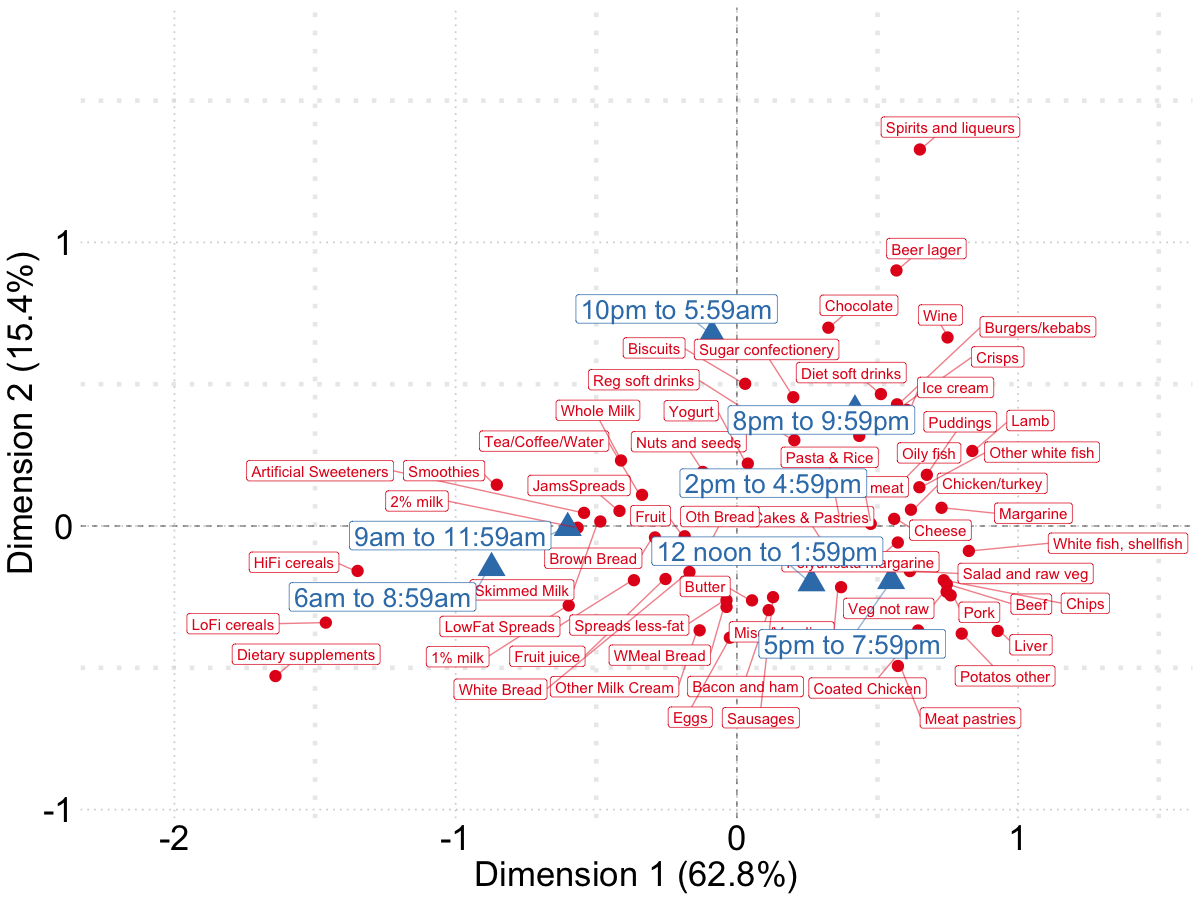
\includegraphics[width=0.88\textwidth]{Fig/F60T7_PreDM}	\vskip-2.45ex
      \label{fig:PreDM}
    \end{figure}
    % \begin{figure}
    %   \centering
    %   \caption{Biplot for CA of 60 food groups and 7 time slots in NDNS RP.}
    %   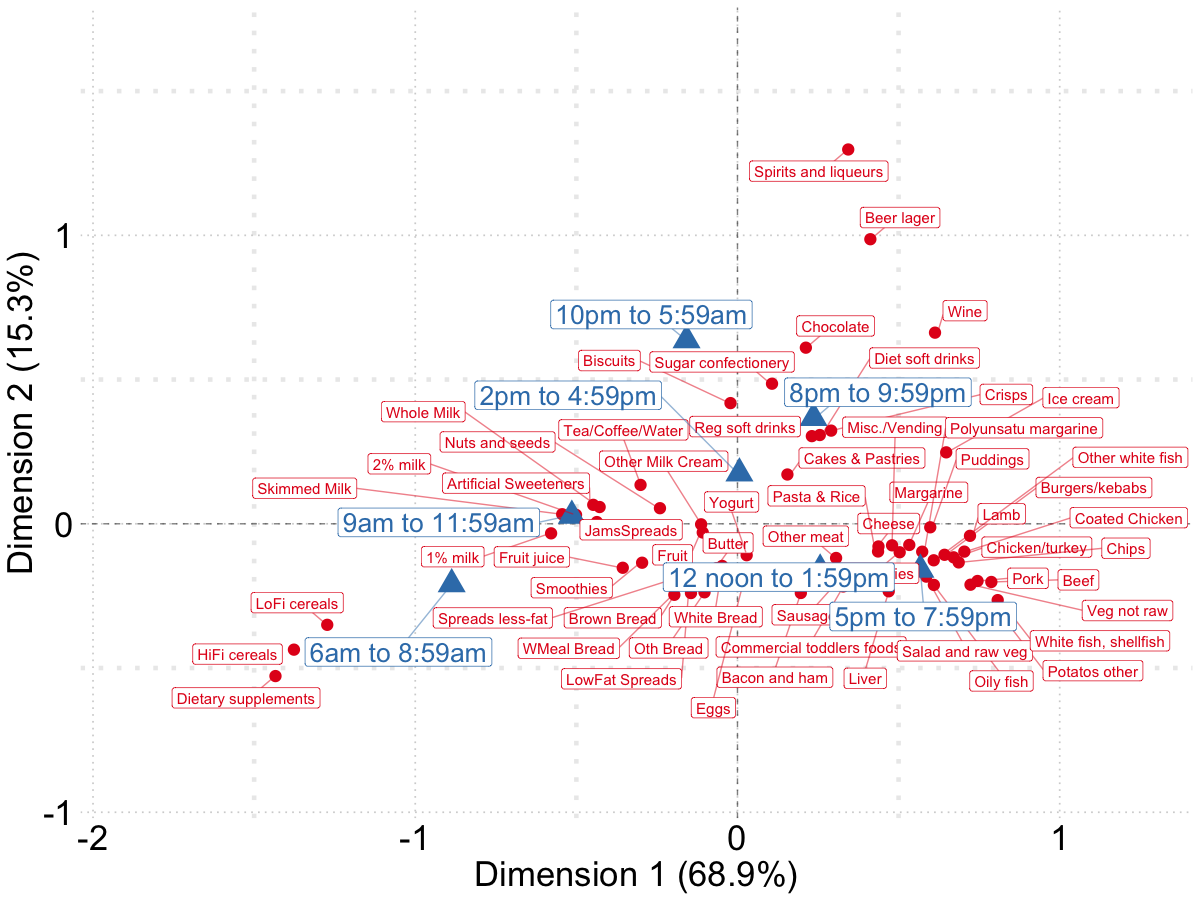
\includegraphics[width=0.95\textwidth]{Fig/F60T7.png}	\vskip-2.45ex
    %   \label{fig:PreDM}
    % \end{figure}
    
    % Please add the following required packages to your document preamble:
% \usepackage{booktabs}
\begin{table}
\caption{\label{tab:tab2}OR (99\%CI) for food groups eaten at night (8pm - ) vs. earlier time, among total and according to different T2D status, NDNS RP 2008-2017.}
\small
\vskip-1.85ex
\begin{tabular}{@{}lccccc@{}}
\toprule
\textbf{Food group}  & \textbf{Overall}    & \textbf{Non-DM}     & \textbf{Pre-DM}    & \textbf{Undiag-DM}  & \textbf{DM}         \\ \midrule
Pudding              & 1.38 (1.03, 1.86)   & 1.50 (1.10, 2.07)   & 0.89 (0.16, 4.87)  & 1.81 (0.41, 7.98)   & 0.58 (0.14, 2.43)   \\
Sweetened Soft drink & 1.74 (1.47, 2.06)   & 1.72 (1.43, 2.06)   & 1.87 (0.97, 3.57)  & 2.72 (1.44, 5.14)   & 1.38 (0.65, 2.96)   \\
Sugar Confectionery  & 1.92 (1.38, 2.69)   & 1.63 (1.14, 2.32)   & 2.10 (0.52, 8.46)  & 13.07 (4.59, 37.24) & 5.10 (2.15, 12.09)  \\
Chocolate            & 3.19 (2.69. 3.79)   & 3.10 (2.57, 3.73)   & 4.07 (2.58, 3.73)  & 2.52 (0.95, 6.66)   & 5.13 (2.55, 10.30)  \\
Spirit               & 11.13 (8.37, 14.80) & 10.86 (8.01, 14.73) & 8.48 (2.26, 31.79) & 7.51 (1.99, 5.21)   & 36.8 (7.36, 183.66) \\
Beer                 & 7.19 (5.87, 8.82)   & 7.49 (6.02, 9.34)   & 4.05 (2.00, 8.20)  & 7.87 (3.51, 17.63)  & 6.32 (2.29, 17.47)  \\
Ice cream            & 2.38 (1.79, 3.15)   & 2.45 (1.82, 3.31)   & 3.32 (0.75, 14.62) & 0.98 (0.14, 7.00)   & 1.65 (0.54, 5.07)   \\
Biscuit              & 1.91 (1.67, 2.16)   & 1.78 (1.55, 2.03)   & 3.51 (2.16, 5.71)  & 2.75 (1.35, 5.59)   & 2.44 (1.54, 3.88)   \\
Crisp                & 1.55 (1.27, 1.88)   & 1.56 (1.27, 1.92)   & 1.95 (0.79, 4.78)  & 1.37 (0.37, 5.12)   & 1.16 (0.49, 2.75)   \\ \bottomrule
\multicolumn{6}{l}{Mixed effect logisitic regression models were adjusted for age, sex, and social-economic status.}\\
\end{tabular}
\end{table}

    
    
  \end{block}



\begin{block}{Discussion}


\begin{itemize}
\item Assessing the relationships between less healthy foods and timing of eating is a first step towards identifying specific public health targets for behaviour change/modification.
\item All unhealthy foods emerged from CA were significantly more likely to be eaten after 8pm. These included alcoholic/sweetened beverages, chocolates and other foods rich in added sugars and saturated fats like biscuits and ice-cream.
\item Food and drinks consumed in the evening/night time slot tend to be highly processed and easily accessible.
\item Undiagnosed T2D patients might be at higher risk of causing/worsening their condition as they had higher odds to consume a number of less healthy foods after 8pm (sugar-confectionary, biscuits, sweetened soft drinks and puddings) than diabetics and non diabetics.
\item The survey cross-sectional nature warrants further investigations by longitudinal cohort studies to establish the causal relation between time of eating of unhealthy foods and diabetes.

\end{itemize}

\end{block}


\end{column}

\separatorcolumn
\end{columns}



% \someheading{Discussion}
% \par
% \begingroup
% \leftskip2em
% \rightskip\leftskip
% \somebody{The high-CH eaters profile seemed to be the healthiest. Low-CH eating which was crudely associated with higher prevalence of hypertension and obesity may have resulted from health/weight concerns, leading to fat or alcohol as replacements for CH. To ascertain the direction of causality in the association of CH patterns with blood pressure and obesity, prospective longitudinal studies are warranted. }
% \par
% \endgroup

\noindent\textcolor{steelblue}{\rule{\textwidth}{0.4pt}}
%  \begin{block}{References}
    \vskip-1.25ex
%    \nocite{*}
    \footnotesize{\bibliographystyle{elsarticle-num}\bibliography{poster}}

%  \end{block}

%\end{column}
%
%\separatorcolumn
%\end{columns}
%\end{frame}
\end{frame}
\end{document}
